\chapter{有限元方法}
\label{chap:appendix-b}

\begin{note}[内容提要]\label{note:appendix-b-1}
本附录简要介绍有限元方法.特别地,这里将引入本书中通用的记号,并说明若干对不可压缩流问题离散化很重要的有限元空间.
\end{note}
\index{有限元方法}

\section{Ritz 方法与 Galerkin 方法}\label{sec:appendix-b-1}

\begin{note}[内容提要]\label{note:appendix-b-2}
本节研究 Hilbert 空间中的抽象问题,并讨论解的存在性与唯一性.用有限维空间逼近解的方法称为 Ritz 方法或 Galerkin 方法;本节还将证明该方法的一些基本性质.本节考虑 Hilbert 空间 $V$,其内积记为
$a(\cdot,\cdot):V\times V\to\mathbb R$,诱导范数为
$\|v\|_V=a(v,v)^{1/2}$.
\end{note}
\index{Ritz 方法}
\index{Galerkin 方法}

\begin{theorem}[Riesz 表示定理]\label{thm:appendix-b-3}
设 $f\in V'$ 是连续线性泛函,则存在唯一确定的 $u\in V$,使得
\begin{equation}\label{eq:appendix-b-1}
 a(u,v)=f(v)\qquad \forall v\in V.
\end{equation}
此外,$u$ 也是如下变分问题的唯一解:
\begin{equation}\label{eq:appendix-b-2}
 \mathcal F(v)=\frac12a(v,v)-f(v)\longrightarrow
 \min_{v\in V}.
\end{equation}
\end{theorem}
\begin{proof}
先证明变分问题存在解.由于 $f$ 连续,存在常数 $c>0$,使得
$|f(v)|\le c\|v\|_V$ 对所有 $v\in V$ 成立.因此
\[
 \mathcal F(v)\ge \frac12\|v\|_V^2-c\|v\|_V
 \ge -\frac12c^2,
\]
其中第二个不等式可由对二次函数 $\frac12t^2-ct$ 求极小得到.于是函数 $\mathcal F(\cdot)$ 有下界,且
\[
 d=\inf_{v\in V}\mathcal F(v)
\]
存在.取序列 $\{v_k\}_{k\in\mathbb N}$,使得 $k\to\infty$ 时
$\mathcal F(v_k)\to d$.由 Hilbert 空间中的平行四边形恒等式可得
\[
 \|v_k-v_l\|_V^2+\|v_k+v_l\|_V^2
 =2\|v_k\|_V^2+2\|v_l\|_V^2.
\]
利用 $f(\cdot)$ 的线性以及对所有 $v\in V$ 均有 $d\le\mathcal F(v)$,得到
\begin{align*}
 \|v_k-v_l\|_V^2
 &=2\|v_k\|_V^2+2\|v_l\|_V^2
   -4\left\|\frac{v_k+v_l}{2}\right\|_V^2\\
 &=4\mathcal F(v_k)+4\mathcal F(v_l)
   -8\mathcal F\left(\frac{v_k+v_l}{2}\right)\\
 &\le 4\mathcal F(v_k)+4\mathcal F(v_l)-8d
 \longrightarrow 0,\qquad k,l\to\infty.
\end{align*}
所以 $\{v_k\}_{k\in\mathbb N}$ 是 Cauchy 序列.由于 $V$ 完备,存在该序列的极限 $u\in V$,参见定义\hyperref[def:appendix-a-5]{A.5}.又因 $\mathcal F(\cdot)$ 连续,$\mathcal F(u)=d$,故 $u$ 是变分问题的解.

接下来证明变分问题\hyperref[eq:appendix-b-2]{(B.2)} 的每个解都是式\hyperref[eq:appendix-b-1]{(B.1)} 的解.令
\[
\begin{aligned}
 \phi(\varepsilon)
 &=\mathcal F(u+\varepsilon v)
 =\frac12a(u+\varepsilon v,u+\varepsilon v)-f(u+\varepsilon v)\\
 &=\frac12a(u,u)+\varepsilon a(u,v)
   +\frac{\varepsilon^2}{2}a(v,v)-f(u)-\varepsilon f(v).
\end{aligned}
\]
若 $u$ 是变分问题的极小点,则函数 $\phi(\varepsilon)$ 在 $\varepsilon=0$ 处有局部极小值.局部极小值的必要条件给出
\[
 0=\phi'(0)=a(u,v)-f(v)\qquad \forall v\in V,
\]
即式\hyperref[eq:appendix-b-1]{(B.1)}.

最后证明解的唯一性.只需证明式\hyperref[eq:appendix-b-1]{(B.1)} 的解唯一:若它有唯一解,则由前一步可知,变分问题\hyperref[eq:appendix-b-2]{(B.2)} 不可能有两个不同的解.设 $u_1,u_2$ 是式\hyperref[eq:appendix-b-1]{(B.1)} 的两个解.两式相减得
\[
 a(u_1-u_2,v)=0\qquad \forall v\in V.
\]
特别取 $v=u_1-u_2$,便有 $\|u_1-u_2\|_V=0$,从而 $u_1=u_2$.
\end{proof}


\index{Riesz 表示定理}

\begin{theorem}[Lax--Milgram 定理]\label{thm:appendix-b-4}
设 $b(\cdot,\cdot):V\times V\to\mathbb R$ 是 Hilbert 空间 $V$ 上有界且强制的双线性型.则对每个有界线性泛函 $f\in V'$,恰有一个 $u\in V$ 满足
\begin{equation}\label{eq:appendix-b-3}
 b(u,v)=f(v)\qquad \forall v\in V.
\end{equation}
\end{theorem}
\begin{proof}
定义线性算子 $T,T':V\to V$,使得
\begin{equation}\label{eq:appendix-b-4}
 a(Tu,v)=b(u,v)\quad\forall v\in V,\qquad
 a(T'u,v)=b(v,u)\quad\forall v\in V.
\end{equation}
由于 $b(u,\cdot)$ 与 $b(\cdot,u)$ 都是 $V$ 上的连续线性泛函,由 Riesz 表示定理\hyperref[thm:appendix-b-3]{B.3} 可知,元素 $Tu$ 与 $T'u$ 存在且唯一.算子满足
\begin{equation}\label{eq:appendix-b-5}
 a(Tu,v)=b(u,v)=a(T'v,u)=a(u,T'v),
\end{equation}
所以 $T'$ 是 $T$ 的伴随算子.令式\hyperref[eq:appendix-b-4]{(B.4)} 中的 $v=Tu$,并利用 $b(\cdot,\cdot)$ 的有界性,可得
\[
\begin{aligned}
 \|Tu\|_V^2&=a(Tu,Tu)=b(u,Tu)
 \le M\|u\|_V\|Tu\|_V,\\
 &\Longrightarrow\quad \|Tu\|_V\le M\|u\|_V.
\end{aligned}
\]
对所有 $u\in V$ 成立.因此 $T$ 有界.由于 $T$ 是线性算子,它也是连续的,参见引理\hyperref[lem:appendix-a-62]{A.62}.同理可证 $T'$ 也有界且连续.

定义双线性型
\[
 d(u,v):=a(TT'u,v)=a(T'u,T'v)\qquad \forall u,v\in V,
\]
其中第二个等号由式\hyperref[eq:appendix-b-5]{(B.5)} 得到.因此 $d(\cdot,\cdot)$ 是对称的.利用 $b(\cdot,\cdot)$ 的强制性及 Cauchy--Schwarz 不等式\hyperref[lem:appendix-a-13]{A.13},有
\[
 m^2\|v\|_V^4
 \le b(v,v)^2
 =a(T'v,v)^2
 \le \|v\|_V^2\|T'v\|_V^2
 =\|v\|_V^2d(v,v).
\]
再利用 $T'$ 的有界性,得到
\begin{equation}\label{eq:appendix-b-6}
 m^2\|v\|_V^2\le d(v,v)\le \|T'\|^2\|v\|_V^2.
\end{equation}
因此 $d(\cdot,\cdot)$ 也是强制的;又因它对称,故定义了 $V$ 上的一个内积.由式\hyperref[eq:appendix-b-6]{(B.6)} 可知,$d(v,v)^{1/2}$ 所诱导的范数与 $\|v\|_V$ 等价.因此,$V$ 在该内积下仍为 Hilbert 空间.再由 Riesz 表示定理\hyperref[thm:appendix-b-3]{B.3},存在唯一的 $w\in V$,使得
\[
 d(w,v)=f(v)\qquad \forall v\in V.
\]
在式\hyperref[eq:appendix-b-3]{(B.3)} 中取 $u=T'w$,并利用式\hyperref[eq:appendix-b-4]{(B.4)},可得
\[
 b(T'w,v)=a(TT'w,v)=d(w,v)=f(v)\qquad \forall v\in V.
\]
因此 $u=T'w$ 是式\hyperref[eq:appendix-b-3]{(B.3)} 的一个解.解的唯一性可仿照对称情形证明.
\end{proof}
\index{Lax--Milgram 定理}

\begin{note}[Ritz 方法的基本思想]\label{note:appendix-b-5}
为了用数值方法逼近式\hyperref[eq:appendix-b-2]{(B.2)} 或式\hyperref[eq:appendix-b-1]{(B.1)} 的解,假设 $V$ 有可数正交归一基(Schauder 基),即 $V$ 是可分 Hilbert 空间.由 Parseval 等式可知,存在有限维子空间 $V_1,V_2,\ldots\subset V$,满足 $\dim V_k=k$,并具有如下性质:对每个 $u\in V$ 及每个 $\varepsilon>0$,存在 $K\in\mathbb N$ 和 $u_k\in V_k$,使得
\begin{equation}\label{eq:appendix-b-7}
 \|u-u_k\|_V\le\varepsilon\qquad \forall k\ge K.
\end{equation}
注意,这里并未要求 $V_k\subseteq V_{k+1}$.

式\hyperref[eq:appendix-b-2]{(B.2)} 与式\hyperref[eq:appendix-b-1]{(B.1)} 的 Ritz 近似定义如下:求 $u_k\in V_k$,使得
\begin{equation}\label{eq:appendix-b-8}
 a(u_k,v_k)=f(v_k)\qquad \forall v_k\in V_k.
\end{equation}
\end{note}
\index{Ritz 方法}
\index{有限维空间!最佳逼近}

\begin{lemma}[式(B.8)解的存在唯一性]\label{lem:appendix-b-6}
式\hyperref[eq:appendix-b-8]{(B.8)} 恰有一个解.
\end{lemma}
\begin{proof}
Hilbert 空间的有限维子空间本身也是 Hilbert 空间,因此可将 Riesz 表示定理\hyperref[thm:appendix-b-3]{B.3} 应用于式\hyperref[eq:appendix-b-8]{(B.8)},即得本引理结论.此外,式\hyperref[eq:appendix-b-8]{(B.8)} 的解也使限制在 $V_k$ 上的一个极小化问题取得极小值.
\end{proof}
\index{Ritz 方法!最佳逼近性质}

\begin{lemma}[最佳逼近性质]\label{lem:appendix-b-7}
式\hyperref[eq:appendix-b-8]{(B.8)} 的解是 $u$ 在 $V_k$ 中的最佳逼近,即
\begin{equation}\label{eq:appendix-b-9}
 \|u-u_k\|_V=\inf_{v_k\in V_k}\|u-v_k\|_V.
\end{equation}
\end{lemma}
\begin{proof}
由于 $V_k\subseteq V$,可在弱方程\hyperref[eq:appendix-b-1]{(B.1)} 中取来自 $V_k$ 的试验函数.将式\hyperref[eq:appendix-b-1]{(B.1)} 与式\hyperref[eq:appendix-b-8]{(B.8)} 相减,得到正交性关系,也称为 Galerkin 正交性:
\begin{equation}\label{eq:appendix-b-10}
 a(u-u_k,v_k)=0\qquad \forall v_k\in V_k.
\end{equation}
因此误差 $u-u_k$ 与子空间 $V_k$ 正交,即 $u-u_k\perp V_k$.换言之,$u_k$ 是 $u$ 关于 $V$ 内积在 $V_k$ 上的正交投影.

任取 $w_k\in V_k$,令 $v_k=u_k-w_k\in V_k$.由 Galerkin 正交性\hyperref[eq:appendix-b-10]{(B.10)} 及 Cauchy--Schwarz 不等式\hyperref[lem:appendix-a-13]{A.13},有
\[
 \|u-u_k\|_V^2
 =a(u-u_k,u-u_k)
 =a(u-u_k,u-v_k)
 \le \|u-u_k\|_V\|u-v_k\|_V.
\]
由于 $w_k$ 任意,$v_k$ 也任意.若 $\|u-u_k\|_V>0$,两边除以此范数即得结论;若 $\|u-u_k\|_V=0$,结论显然成立.
\end{proof}
\index{Ritz 方法!收敛性}

\begin{theorem}[Ritz 近似的收敛性]\label{thm:appendix-b-8}
Ritz 近似收敛,即
\[
 \lim_{k\to\infty}\|u-u_k\|_V=0.
\]
\end{theorem}
\begin{proof}
由最佳逼近性质\hyperref[lem:appendix-b-7]{引理 B.7} 及性质\hyperref[eq:appendix-b-7]{(B.7)},对每个 $\varepsilon>0$ 及所有 $k\ge K(\varepsilon)$,均有
\[
 \|u-u_k\|_V=\inf_{v_k\in V_k}\|u-v_k\|_V\le\varepsilon.
\]
因此收敛性得证.
\end{proof}

\begin{note}[将 Ritz 方法写成线性方程组]\label{note:appendix-b-9}
计算 $u_k$ 时,可以选取 $V_k$ 的任意一组基 $\{\phi_i\}_{i=1}^k$.式\hyperref[eq:appendix-b-8]{(B.8)} 对所有 $v_k\in V_k$ 成立,当且仅当它对每个基函数 $\phi_i$ 成立.这是因为等式两边关于试验函数都是线性的,且 $V_k$ 中任一元素都能表示为基函数的线性组合.令
$v_k=\sum_{i=1}^k\alpha_i\phi_i$,则由式\hyperref[eq:appendix-b-8]{(B.8)} 得
\[
 a(u_k,v_k)=\sum_{i=1}^k\alpha_i a(u_k,\phi_i)
 =\sum_{i=1}^k\alpha_i f(\phi_i)=f(v_k).
\]
这说明,只要 $a(u_k,\phi_i)=f(\phi_i)$ 对 $i=1,\ldots,k$ 成立,式\hyperref[eq:appendix-b-8]{(B.8)} 就成立;反过来,若式\hyperref[eq:appendix-b-8]{(B.8)} 成立,它当然也对每个基函数 $\phi_i$ 成立.

将近似解写成基函数的线性组合
\[
 u_k=\sum_{j=1}^k u_j\phi_j,
\]
其中系数 $u_j\in\mathbb R$ 未知.取基函数作为试验函数,得到
\[
 \sum_{j=1}^k a(u_j\phi_j,\phi_i)
 =\sum_{j=1}^k a(\phi_j,\phi_i)u_j
 =f(\phi_i),\qquad i=1,\ldots,k.
\]
该式等价于线性方程组 $Au=f$,其中
\[
 A=(a_{ij})_{i,j=1}^k
   =\bigl(a(\phi_j,\phi_i)\bigr)_{i,j=1}^k
\]
称为刚度矩阵.注意,矩阵元素的下标顺序与内积两个自变量的顺序不同.右端向量 $f$ 的长度为 $k$,其分量为 $f_i=f(\phi_i)$,$i=1,\ldots,k$.

利用系数向量 $(v_1,\ldots,v_k)^{\mathsf T}$ 与元素
$v_k=\sum_{i=1}^k v_i\phi_i$ 之间的一一对应关系,可证明矩阵 $A$ 对称正定,当且仅当
\[
\begin{aligned}
 A=A^{\mathsf T}
 &\quad\Longleftrightarrow\quad
 a(v,w)=a(w,v)\qquad \forall v,w\in V_k,\\
 x^{\mathsf T}Ax>0\ \ \forall x\ne0
 &\quad\Longleftrightarrow\quad
 a(v,v)>0\qquad \forall v\in V_k\setminus\{0\}.
\end{aligned}
\]
\end{note}
\index{Ritz 方法!刚度矩阵}

\begin{note}[有界强制双线性型的情形]\label{note:appendix-b-10}
若 $b(\cdot,\cdot)$ 有界且强制,但不对称,则仍可用与 Ritz 方法相同的思路逼近式\hyperref[eq:appendix-b-3]{(B.3)} 的解;此时称为 Galerkin 方法.离散问题为:求 $u_k\in V_k$,使得
\begin{equation}\label{eq:appendix-b-11}
 b(u_k,v_k)=f(v_k)\qquad \forall v_k\in V_k.
\end{equation}
\end{note}
\index{Galerkin 方法}

\begin{lemma}[式(B.11)解的存在唯一性]\label{lem:appendix-b-11}
式\hyperref[eq:appendix-b-11]{(B.11)} 恰有一个解.
\end{lemma}
\begin{proof}
本引理直接由 Lax--Milgram 定理\hyperref[thm:appendix-b-4]{B.4} 得出.
\end{proof}

\begin{lemma}[Céa 引理(误差估计)]\label{lem:appendix-b-12}\label{lem:cea}
设 $b:V\times V\to\mathbb R$ 是 Hilbert 空间 $V$ 上有界且强制的双线性型,$f\in V'$ 是有界线性泛函.令 $u$ 为式\hyperref[eq:appendix-b-3]{(B.3)} 的解,$u_k$ 为式\hyperref[eq:appendix-b-11]{(B.11)} 的解,则有误差估计
\begin{equation}\label{eq:appendix-b-12}
 \|u-u_k\|_V\le\frac{M}{m}\inf_{v_k\in V_k}\|u-v_k\|_V,
\end{equation}
其中常数 $M$ 和 $m$ 由式\hyperref[eq:appendix-a-47]{(A.47)} 与式\hyperref[eq:appendix-a-48]{(A.48)} 给出.
\end{lemma}
\begin{proof}
将连续方程\hyperref[eq:appendix-b-3]{(B.3)} 与离散方程\hyperref[eq:appendix-b-11]{(B.11)} 相减,得到误差方程
\[
 b(u-u_k,v_k)=0\qquad \forall v_k\in V_k,
\]
这也称为 Galerkin 正交性.由强制性、Galerkin 正交性以及有界性\hyperref[eq:appendix-a-48]{(A.48)}、\hyperref[eq:appendix-a-47]{(A.47)},对任意 $v_k\in V_k$ 有
\[
\begin{aligned}
 \|u-u_k\|_V^2
 &\le \frac1m b(u-u_k,u-u_k)
 =\frac1m b(u-u_k,u-v_k)\\
 &\le \frac{M}{m}\|u-u_k\|_V\|u-v_k\|_V.
\end{aligned}
\]
若 $\|u-u_k\|_V>0$,约去该因子并对 $v_k$ 取下确界,即得式\hyperref[eq:appendix-b-12]{(B.12)};若误差为零,结论显然成立.
\end{proof}
\index{Céa 引理}
\index{Galerkin 正交性}

\begin{note}[最佳逼近误差]\label{note:appendix-b-13}
由误差估计\hyperref[eq:appendix-b-12]{(B.12)} 可知,误差被最佳逼近误差的一个倍数所控制,而该倍数取决于双线性型 $b(\cdot,\cdot)$ 的性质.因此,在研究具体有限维空间的误差估计时,最佳逼近误差的分析十分重要.
\end{note}
\index{最佳逼近误差}

\begin{note}[相应的线性方程组]\label{note:appendix-b-14}
相应的线性方程组可仿照对称情形推导.所得系统矩阵仍为正定矩阵,但不再对称.
\end{note}

\begin{lemma}[有限维空间的 inf-sup 判据]\label{lem:appendix-b-15}
设 $V^h$ 是带内积 $(\cdot,\cdot)_{V^h}$ 的有限维空间,其诱导范数为
$\|v^h\|_{V^h}=(v^h,v^h)_{V^h}^{1/2}$.考虑双线性型
$a:V^h\times V^h\to\mathbb R$ 与线性泛函 $f:V^h\to\mathbb R$.则问题:求 $u^h\in V^h$,使得
\begin{equation}\label{eq:appendix-b-13}
 a(u^h,v^h)=f(v^h)\qquad \forall v^h\in V^h
\end{equation}
对所有 $f(\cdot)$ 都有唯一解,当且仅当
\begin{equation}\label{eq:appendix-b-14}
 \inf_{w^h\in V^h\setminus\{0\}}\ 
 \sup_{v^h\in V^h\setminus\{0\}}
 \frac{a(v^h,w^h)}{\|v^h\|_{V^h}\|w^h\|_{V^h}}
 \ge \beta_{\mathrm{ish}}^h>0.
\end{equation}
\end{lemma}
\index{inf-sup 条件!有限维空间判据}
\begin{proof}
记 $n\in\mathbb N$ 为 $V^h$ 的维数,并令 $\{\phi_i^h\}_{i=1}^n$ 为 $V^h$ 的一组基.写成
\[
 v^h=\sum_{i=1}^n v_i\phi_i^h,\qquad
 w^h=\sum_{i=1}^n w_i\phi_i^h,
\]
其中 $v=(v_1,\ldots,v_n)^{\mathsf T}$、$w=(w_1,\ldots,w_n)^{\mathsf T}$.存在矩阵 $A,M\in\mathbb R^{n\times n}$,使得
\[
\begin{aligned}
 a(v^h,w^h)&=v^{\mathsf T}A^{\mathsf T}w,\\
 \|v^h\|_{V^h}&=(v^{\mathsf T}M^{\mathsf T}v)^{1/2},\\
 \|w^h\|_{V^h}&=(w^{\mathsf T}M^{\mathsf T}w)^{1/2}.
\end{aligned}
\]
矩阵 $M$ 对称正定.因此 inf-sup 条件\hyperref[eq:appendix-b-14]{(B.14)} 可写成
\begin{equation}\label{eq:appendix-b-15}
 \inf_{w\in\mathbb R^n\setminus\{0\}}\ 
 \sup_{v\in\mathbb R^n\setminus\{0\}}
 \frac{v^{\mathsf T}A^{\mathsf T}w}
 {(v^{\mathsf T}Mv)^{1/2}(w^{\mathsf T}Mw)^{1/2}}
 \ge\beta_{\mathrm{ish}}^h>0.
\end{equation}
问题\hyperref[eq:appendix-b-13]{(B.13)} 对每个 $f$ 都有唯一解,当且仅当矩阵 $A$ 非奇异.

\textbf{(B.15)成立 $\Longrightarrow A$ 非奇异.}
反设 $A$ 奇异,则 $A^{\mathsf T}$ 也奇异,存在 $w\ne0$ 使得 $A^{\mathsf T}w=0$.于是,对该 $w$,式\hyperref[eq:appendix-b-15]{(B.15)} 中关于 $v$ 的上确界为零,这与式\hyperref[eq:appendix-b-15]{(B.15)} 成立矛盾.

\textbf{$A$ 非奇异 $\Longrightarrow$(B.15)成立.}
若 $A$ 非奇异,则 $A^{\mathsf T}$ 也非奇异.对每个 $w\in\mathbb R^n\setminus\{0\}$,在上确界中取
$v=M^{-1}A^{\mathsf T}w$;由于 $M$ 与 $A^{\mathsf T}$ 均非奇异,该向量非零.利用 $M$ 对称正定,便有
\begin{align*}
 \sup_{v\ne0}
 \frac{v^{\mathsf T}A^{\mathsf T}w}
 {(v^{\mathsf T}Mv)^{1/2}(w^{\mathsf T}Mw)^{1/2}}
 &\ge
 \left(\frac{w^{\mathsf T}AM^{-1}A^{\mathsf T}w}
 {w^{\mathsf T}Mw}\right)^{1/2}.
\end{align*}
令 $z=M^{1/2}w$,则右侧平方为矩阵
\[
\begin{aligned}
 S&=M^{-1/2}AM^{-1}A^{\mathsf T}M^{-1/2}\\
 &=CC^{\mathsf T},\qquad
 C=M^{-1/2}AM^{-1/2}.
\end{aligned}
\]
对应的 Rayleigh 商.由引理\hyperref[lem:appendix-a-19]{A.19},Rayleigh 商的下确界可取到,并等于相应特征值问题的最小特征值.矩阵 $S$ 对称;而且
\[
 z^{\mathsf T}Sz
 =\|C^{\mathsf T}z\|_2^2\ge0,
\]
故它半正定,所有特征值均为实数且非负.又因 $A$ 与 $M$ 均非奇异,$C$ 亦非奇异,故 $S=CC^{\mathsf T}$ 实际上正定,所有特征值均为正.因此存在常数 $\beta_{\mathrm{ish}}^h>0$,使得对所有 $w\ne0$,
\[
\begin{aligned}
 \left(\frac{w^{\mathsf T}AM^{-1}A^{\mathsf T}w}
 {w^{\mathsf T}Mw}\right)^{1/2}\\
 \ge\beta_{\mathrm{ish}}^h.
\end{aligned}
\]
于是先对 $w$ 取下确界,再取关于 $v$ 的上确界,只会使左端不减,从而式\hyperref[eq:appendix-b-15]{(B.15)} 成立.
\end{proof}

\section{有限元空间}\label{sec:appendix-b-2}

\begin{note}[网格单元、面、棱与顶点]\label{note:appendix-b-16}
网格单元 $K$ 是 $\mathbb R^d$ 中的紧多面体,其中 $d\in\{2,3\}$,且其内部非空.边界 $\partial K$ 由若干 $m$ 维仿射子流形组成,包括点、直线段及平面片,其中 $0\le m\le d-1$;这些子流形称为 $m$ 维面.$0$ 维面是网格单元的顶点,$1$ 维面是棱,而 $(d-1)$ 维面简称面.
\end{note}
\index{网格单元}
\index{面}
\index{棱}
\index{顶点}

\begin{note}[定义在 $K$ 上的有限维空间]\label{note:appendix-b-17}
设 $s\in\mathbb N$.有限元方法使用定义在 $K$ 上的有限维空间
$P(K)\subset C^s(K)$.通常,$P(K)$ 由多项式组成.$P(K)$ 的维数记为
\[
 \dim P(K)=N_K.
\]
\end{note}
\index{有限维空间}
\index{多项式空间}

\begin{note}[定义在 $P(K)$ 上的线性泛函与节点泛函]\label{note:appendix-b-18}
定义有限元时,定义在 $P(K)$ 上的线性泛函十分重要,这些泛函称为节点泛函.考虑 $N_K$ 个线性连续泛函
\[
 \Phi_{K,1},\ldots,\Phi_{K,N_K}:C^s(K)\to\mathbb R,
\]
并假设它们线性无关.有限元方法中可采用不同类型的泛函:
\begin{itemize}
 \item 点值:$\Phi(v)=v(x)$,其中 $x\in K$;
 \item 一阶偏导数的点值:$\Phi(v)=\partial_i v(x)$,其中 $x\in K$;
 \item $K$ 的面 $E$ 上法向导数的点值:
       $\Phi(v)=\nabla v(x)\cdot n_E$,其中 $n_E$ 是 $E$ 上指向外侧的单位法向量;
 \item 在 $K$ 上的积分平均值:
       $\displaystyle \Phi(v)=\frac1{|K|}\int_K v(x)\,\mathrm dx$;
 \item 在面 $E$ 上的积分平均值:
       $\displaystyle \Phi(v)=\frac1{|E|}\int_E v(s)\,\mathrm ds$.
\end{itemize}
光滑性参数 $s$ 必须选得足够大,以保证泛函
$\Phi_{K,1},\ldots,\Phi_{K,N_K}$ 连续.例如,若某个泛函需要计算偏导数或法向导数,则至少应取 $s=1$;对上面列出的其他泛函,取 $s=0$ 即可.
\end{note}
\index{节点泛函}
\index{法向导数}
\index{积分平均值}

\begin{definition}[关于泛函的唯一确定性]\label{def:appendix-b-19}
若对每个 $a\in\mathbb R^{N_K}$,其中
$a=(a_1,\ldots,a_{N_K})^{\mathsf T}$,都恰有一个 $p\in P(K)$ 满足
\[
 \Phi_{K,i}(p)=a_i,\qquad 1\le i\le N_K,
\]
则称空间 $P(K)$ 关于泛函 $\Phi_{K,1},\ldots,\Phi_{K,N_K}$ 具有唯一确定性.
\end{definition}
\index{唯一确定性}

\begin{note}[局部基函数]\label{note:appendix-b-20}
唯一确定性意味着,对每个向量 $a\in\mathbb R^{N_K}$,其中
$a=(a_1,\ldots,a_{N_K})^{\mathsf T}$,在 $P(K)$ 中恰有一个元素使第 $i$ 个泛函的值为 $a_i$.特别地,依次取 $a$ 为标准基向量,可知存在一组函数
$\{\phi_{K,i}\}_{i=1}^{N_K}$,满足 $\phi_{K,i}\in P(K)$ 且
\[
 \Phi_{K,i}(\phi_{K,j})=\delta_{ij},
 \qquad i,j=1,\ldots,N_K.
\]
因此 $\{\phi_{K,i}\}_{i=1}^{N_K}$ 构成 $P(K)$ 的一组基,称为局部基.
\end{note}
\index{局部基}

\begin{note}[任意基向局部基的转换]\label{note:appendix-b-21}
若已知 $P(K)$ 的任意一组基 $\{p_i\}_{i=1}^{N_K}$,则可通过求解线性方程组计算局部基.为此,将局部基表示为已知基的线性组合
\[
 \phi_{K,j}=\sum_{k=1}^{N_K}c_{jk}p_k,\qquad
 c_{jk}\in\mathbb R,\quad j=1,\ldots,N_K,
\]
其中 $c_{jk}$ 是待求系数.根据局部基的定义,有
\[
\begin{aligned}
\Phi_{K,i}(\phi_{K,j})
 &=\sum_{k=1}^{N_K}c_{jk}a_{ik}
 =\delta_{ij},\qquad i,j=1,\ldots,N_K,\\
 a_{ik}&=\Phi_{K,i}(p_k).
\end{aligned}
\]
由唯一确定性可知,矩阵 $A=(a_{ij})$ 非奇异,故系数 $c_{jk}$ 可被唯一确定.
\end{note}
\index{局部基!基变换}

\begin{note}[剖分、网格与网格单元]\label{note:appendix-b-22}
定义整体有限元空间时,需要将区域 $\Omega$ 分解为多面体 $K$.该分解称为剖分 $\mathcal T^h$,其中的多面体 $K$ 称为网格单元;这些多面体的并称为网格.

若剖分满足下列条件,则称其为可容许剖分,参见\textcite[第 38、51 页]{Ciarlet1978}:
\begin{itemize}
 \item $\Omega=\bigcup_{K\in\mathcal T^h}K$;
 \item 每个网格单元 $K\in\mathcal T^h$ 都是闭集,且内部 $K^\circ$ 非空;
 \item 对不同的网格单元 $K_1,K_2$,有 $K_1^\circ\cap K_2^\circ=\varnothing$;
 \item 对每个 $K\in\mathcal T^h$,其边界 $\partial K$ 都是 Lipschitz 连续的;
 \item 两个网格单元的交集要么为空,要么是它们共有的一个 $m$ 维面,其中 $m\in\{0,\ldots,d-1\}$.
\end{itemize}
\end{note}
\index{剖分!可容许}
\index{网格}

\begin{note}[整体泛函与局部泛函]\label{note:appendix-b-23}
设 $\Phi_1,\ldots,\Phi_N:C^s(\Omega)\to\mathbb R$ 是连续线性泛函,类型与注记\hyperref[note:appendix-b-18]{B.18} 中给出的一致.将这些泛函限制在 $C^s(K)$ 上,得到一组局部泛函
$\Phi_{K,1},\ldots,\Phi_{K,N_K}$,并假设该组局部泛函在 $P(K)$ 上具有唯一确定性.对每个 $i$,将所有满足如下条件的网格单元 $K_j$ 的并记为 $\Omega_i$:存在 $p\in P(K_j)$ 使得 $\Phi_i(p)\ne0$.
\end{note}
\index{整体泛函}
\index{局部泛函}

\begin{example}[$\Omega_i$ 的子区域]\label{ex:appendix-b-24}
考虑二维情形,并设 $\Phi_i$ 是在 $x\in K$ 处取函数节点值的泛函.若 $x\in K^\circ$,则 $\Omega_i=K$.若 $x$ 位于 $K$ 的一条边上但不是顶点,则 $\Omega_i$ 是 $K$ 与另一个边界含有该边的网格单元之并.最后,若 $x$ 是 $K$ 的一个顶点,则 $\Omega_i$ 是所有包含该顶点的网格单元之并.
\end{example}
\index{节点泛函!支集}

\begin{definition}[有限元空间与整体基]\label{def:appendix-b-25}
设函数 $v(x)$ 定义在 $\Omega$ 上,并且对所有 $K\in\mathcal T^h$ 均有
$v|_K\in P(K)$.若对每个泛函 $\Phi_i$,都有
\[
 \Phi_i(v|_{K_1})=\Phi_i(v|_{K_2})
 \qquad \forall K_1,K_2\in\Omega_i,
\]
 则称 $v$ 关于泛函 $\Phi_i$ 连续.空间
\[
 S=\left\{v\in L^\infty(\Omega):
 \begin{gathered}
  v|_K\in P(K)\qquad \forall K\in\mathcal T^h,\\
  \Phi_i(v|_{K_1})=\Phi_i(v|_{K_2}),\\
  \forall i=1,\ldots,N,\quad \forall K_1,K_2\in\Omega_i
 \end{gathered}\right\}
\]
称为有限元空间.

$S$ 的整体基 $\{\phi_j\}_{j=1}^N$ 由下列条件定义:
\[
 \phi_j\in S,\qquad
 \Phi_i(\phi_j)=\delta_{ij},\qquad i,j=1,\ldots,N.
\]
\end{definition}
\index{有限元空间}
\index{整体基}

\begin{note}[整体基函数]\label{note:appendix-b-26}
整体基函数在每个网格单元上都与一个局部基函数重合;这一性质保证整体基函数的唯一性.泛函组 $\{\Phi_i\}_{i=1}^N$ 所定义的连续性条件是否能推出有限元函数本身连续,取决于用于定义有限元空间的泛函类型.
\end{note}
\index{整体基}

\begin{definition}[参数有限元]\label{def:appendix-b-27}
设 $\widehat K$ 为参考网格单元,其局部空间为 $P(\widehat K)$,局部泛函为
$\widehat\Phi_1,\ldots,\widehat\Phi_{N_{\widehat K}}$,并给定一类双射
$\{F_K:\widehat K\to K\}$.若有限元空间满足以下条件,则称其为参数有限元空间:
\begin{itemize}
 \item 映射族 $\{F_K\}$ 的像 $\{K\}$ 构成网格单元集合;
 \item 局部空间取为
\begin{equation}\label{eq:appendix-b-16}
 P(K)=\left\{p:p=\widehat p\circ F_K^{-1},\
 \widehat p\in P(\widehat K)\right\};
 \end{equation}
 \item 局部泛函定义为
\begin{equation}\label{eq:appendix-b-17}
 \Phi_{K,i}(v(x))
 =\widehat\Phi_i\bigl(v(F_K(\widehat x))\bigr),
 \end{equation}
其中 $\widehat x=(\widehat x_1,\ldots,\widehat x_d)^{\mathsf T}$ 是参考网格单元上的坐标,且 $x=F_K(\widehat x)$.
\end{itemize}
\end{definition}
\index{参数有限元}
\index{参考网格单元}

\begin{note}[使用参数有限元的动机]\label{note:appendix-b-28}
定义\hyperref[def:appendix-b-25]{B.25} 中的有限元空间概念十分一般,例如允许采用不同类型的网格单元.然而,无论有限元理论还是有限元方法的实现,只考虑参数有限元都会简单得多.
\end{note}
\index{参数有限元}

\section{单纯形上的有限元}\label{sec:appendix-b-3}

\begin{definition}[$d$ 维单纯形]\label{def:appendix-b-29}
$d$ 维单纯形 $K\subset\mathbb R^d$ 是 $d+1$ 个点
$a_1,\ldots,a_{d+1}\in\mathbb R^d$ 的凸包,这些点构成 $K$ 的顶点.
\end{definition}
\index{单纯形}

\begin{note}[关于 $d$ 维单纯形]\label{note:appendix-b-30}
以下总假设单纯形非退化,即其 $d$ 维测度为正.这等价于下列矩阵非奇异:
\[
 A=
 \begin{pmatrix}
 a_{11}&a_{12}&\cdots&a_{1,d+1}\\
 a_{21}&a_{22}&\cdots&a_{2,d+1}\\
 \vdots&\vdots&\ddots&\vdots\\
 a_{d1}&a_{d2}&\cdots&a_{d,d+1}\\
 1&1&\cdots&1
  \end{pmatrix}.
 \]
其中
\[
 \bm a_i=(a_{1i},a_{2i},\ldots,a_{di})^{\mathsf T},
 \qquad i=1,\ldots,d+1.
\]
当 $d=2$ 时,单纯形是三角形;当 $d=3$ 时,单纯形是四面体.
\end{note}
\index{单纯形!非退化}

\begin{definition}[重心坐标]\label{def:appendix-b-31}
由于 $K$ 是点集 $\{a_i\}_{i=1}^{d+1}$ 的凸包,利用顶点的凸组合可将 $K$ 参数化为
\[
 K=\left\{\bm x\in\mathbb R^d:
 \bm x=\sum_{i=1}^{d+1}\lambda_i\bm a_i,\quad
 0\le\lambda_i\le1,\quad
 \sum_{i=1}^{d+1}\lambda_i=1\right\}.
\]
系数 $\lambda_1,\ldots,\lambda_{d+1}$ 称为 $\bm x\in K$ 的重心坐标.
\end{definition}
\index{重心坐标}

\begin{note}[关于重心坐标]\label{note:appendix-b-32}
由定义可知,重心坐标是下列线性方程组的解:
\[
 \sum_{i=1}^{d+1}a_{ji}\lambda_i=x_j,\qquad
 1\le j\le d,\qquad
 \sum_{i=1}^{d+1}\lambda_i=1.
\]
由注记\hyperref[note:appendix-b-30]{B.30} 可知,该方程组的系数矩阵非奇异,因此重心坐标唯一确定.

单纯形的顶点 $\bm a_i$ 的重心坐标为 $\lambda_i=1$,且当 $j\ne i$ 时 $\lambda_j=0$.由于 $\lambda_i(\bm a_j)=\delta_{ij}$,坐标函数 $\lambda_i$ 可视为一个线性函数:它在顶点 $\bm a_i$ 处取值 $1$,并在其余顶点 $\bm a_j$($j\ne i$)处取值 $0$.

单纯形的重心为
\[
 \bm S_K=\frac1{d+1}\sum_{i=1}^{d+1}\bm a_i
 =\sum_{i=1}^{d+1}\frac1{d+1}\bm a_i.
\]
因此它的重心坐标为
$\lambda_i=1/(d+1)$,$i=1,\ldots,d+1$.
\end{note}
\index{重心坐标}
\index{重心}

\begin{note}[单纯形的参考网格单元]\label{note:appendix-b-33}
三角形与四面体常用的参考网格单元是单位单纯形
\[
 \widehat K=
 \left\{\widehat{\bm x}\in\mathbb R^d:
 \sum_{i=1}^d\widehat x_i\le1,\quad
 \widehat x_i\ge0,\quad i=1,\ldots,d\right\},
\]
见图\hyperref[fig:appendix-b-1]{B.1}.可容许映射族 $\{F_K\}$ 由双射仿射映射组成:
\begin{equation}\label{eq:appendix-b-18}
 F_K(\widehat{\bm x})=B_K\widehat{\bm x}+\bm b,\qquad
 B_K\in\mathbb R^{d\times d},\quad
 \det(B_K)\ne0,\quad \bm b\in\mathbb R^d.
\end{equation}
这些映射的像构成非退化单纯形 $K\subset\mathbb R^d$ 的集合.
\end{note}
\index{参考网格单元}
\index{单位单纯形}

\begin{definition}[单纯形有限元的仿射族]\label{def:appendix-b-34}
给定单纯形参考网格单元 $\widehat K$、仿射映射族 $\{F_K\}$ 以及定义在 $\widehat K$ 上的一组具有唯一确定性的泛函.利用式\hyperref[eq:appendix-b-16]{(B.16)} 与式\hyperref[eq:appendix-b-17]{(B.17)},可在每个非退化单纯形上得到一个局部有限元空间.所有这些局部空间构成的集合称为单纯形有限元的仿射族.
\end{definition}

\begin{elegantfigure}[0.9\linewidth]
 \centering
 \includegraphics[page=719,pagebox=cropbox,trim=79.50bp 114.40bp 79.61bp 407.75bp,clip,width=\linewidth]{../input/source/Finite Element Methods for Incompressible Flow Problems.pdf}
 \captionof{figure}{二维与三维中的单位单纯形.}\label{fig:appendix-b-1}
\end{elegantfigure}

\begin{definition}[多项式空间 $P_k$]\label{def:appendix-b-35}
设 $\bm x=(x_1,\ldots,x_d)^{\mathsf T}$,$k\in\mathbb N\cup\{0\}$,并令
$\alpha=(\alpha_1,\ldots,\alpha_d)^{\mathsf T}$ 为多重指标.多项式空间 $P_k$ 定义为
\[
 P_k=\operatorname{span}\left\{
 \bm x^\alpha=\prod_{i=1}^d x_i^{\alpha_i}:
 \begin{array}{l}
 \alpha_i\in\mathbb N\cup\{0\},\quad i=1,\ldots,d,\\
 \displaystyle\sum_{i=1}^d\alpha_i\le k
 \end{array}\right\}.
\]
\end{definition}
\index{多项式空间!$P_k$}

\begin{note}[Lagrange 有限元]\label{note:appendix-b-36}
下面许多例子中,定义在参考网格单元 $\widehat K$ 上的线性泛函取值于具有与一般网格单元 $K$ 上相同重心坐标的点.若有限元的线性泛函是对 $K$ 中某些点处的函数值进行取值,则称其为 Lagrange 有限元.
\end{note}
\index{Lagrange 有限元}

\begin{example}[$P_0$:分片常数有限元]\label{ex:appendix-b-37}
分片常数有限元空间由不连续函数组成.其线性泛函是在网格单元重心处取多项式的函数值,见图\hyperref[fig:appendix-b-2]{B.2}.并且
$\dim P_0(K)=1$.
\end{example}
\index{有限元!分片常数}

\begin{elegantfigure}[0.9\linewidth]
 \centering
 \includegraphics[page=720,pagebox=cropbox,trim=79.00bp 481.65bp 79.36bp 60.75bp,clip,width=\linewidth]{../input/source/Finite Element Methods for Incompressible Flow Problems.pdf}
 \captionof{figure}{有限元 $P_0(K)$.}\label{fig:appendix-b-2}
\end{elegantfigure}

\begin{example}[$P_1$:协调分片线性有限元]\label{ex:appendix-b-38}
该有限元空间是 $C(\overline\Omega)$ 的子空间.线性泛函是在网格单元的顶点处取函数值,见图\hyperref[fig:appendix-b-3]{B.3}.因此
$\dim P_1(K)=d+1$.
\begin{elegantfigure}[0.9\linewidth]
 \centering
 \includegraphics[page=721,pagebox=cropbox,trim=79.00bp 475.15bp 79.86bp 60.50bp,clip,width=\linewidth]{../input/source/Finite Element Methods for Incompressible Flow Problems.pdf}
 \captionof{figure}{有限元 $P_1(K)$.}\label{fig:appendix-b-3}
\end{elegantfigure}
对于泛函组 $\{\Phi_i(v)=v(\bm a_i),\ i=1,\ldots,d+1\}$,局部基为
$\{\lambda_i\}_{i=1}^{d+1}$,因为 $\Phi_i(\lambda_j)=\delta_{ij}$,参见注记\hyperref[note:appendix-b-32]{B.32}.既然局部基存在,这些泛函关于多项式空间 $P_1(K)$ 具有唯一确定性.

下面证明相应有限元空间由连续函数组成.设两个网格单元 $K_1,K_2$ 共有一个面 $E$,并令 $v\in S$,其中 $v|_{K_1},v|_{K_2}\in P_1(K_1),P_1(K_2)$.$v|_{K_1}$ 与 $v|_{K_2}$ 在 $E$ 上的限制都是线性函数.需要证明这两个线性函数相同.$(d-1)$ 维面 $E$ 上的线性函数由定义在 $E$ 上的 $d$ 个线性无关泛函唯一确定;这些泛函可取为在 $E$ 的 $d$ 个顶点处取函数值.根据有限元空间 $S$ 的定义,这些泛函是连续的,因此两个限制函数在 $E$ 的各顶点处取值相同.故
$v|_{K_1}|_E=v|_{K_2}|_E$,从而 $P_1$ 有限元函数连续.
\end{example}
\index{有限元!协调分片线性}

\begin{example}[$P_2$:协调分片二次有限元]\label{ex:appendix-b-39}
该有限元空间也是 $C(\overline\Omega)$ 的子空间,由分片二次函数组成.泛函是在网格单元的 $d+1$ 个顶点以及各条棱的中点取函数值,见图\hyperref[fig:appendix-b-4]{B.4}.由于每个顶点都与其余各顶点相连,棱的条数为
$\sum_{i=1}^d i=d(d+1)/2$.因此
\[
 \dim P_2(K)=\frac{(d+1)(d+2)}2.
\]

与顶点泛函 $\{\Phi_i(v)=v(\bm a_i),\ i=1,\ldots,d+1\}$ 对应的局部基部分为
\[
 \left\{\phi_i(\lambda)=\lambda_i(2\lambda_i-1),\
 i=1,\ldots,d+1\right\}.
\]
记顶点 $\bm a_i$ 与 $\bm a_j$ 之间棱的中点为 $\bm a_{ij}$.与这些棱中点泛函对应的局部基部分为
\[
 \left\{\phi_{ij}=4\lambda_i\lambda_j,\
 i,j=1,\ldots,d+1,\ i<j\right\}.
\]
由于局部基存在,唯一确定性成立.相应有限元空间的连续性可仿照 $P_1$ 有限元证明:网格单元上二次函数在面 $E$ 上的限制仍是 $E$ 上的二次函数.因此,面上的函数由 $d(d+1)/2$ 个线性无关泛函唯一确定.
\end{example}
\index{有限元!协调分片二次}

\begin{elegantfigure}[0.9\linewidth]
 \centering
 \includegraphics[page=721,pagebox=cropbox,trim=79.00bp 316.65bp 79.86bp 219.00bp,clip,width=\linewidth]{../input/source/Finite Element Methods for Incompressible Flow Problems.pdf}
 \captionof{figure}{有限元 $P_2(K)$.}\label{fig:appendix-b-4}
\end{elegantfigure}

\begin{example}[$P_3$:协调分片三次有限元]\label{ex:appendix-b-40}
该有限元空间由连续的分片三次函数组成,是 $C(\overline\Omega)$ 的子空间.网格单元 $K$ 上的泛函是在顶点处取值(共 $d+1$ 个),在每条棱上取两个值(将棱三等分,共 $2\sum_{i=1}^d i=d(d+1)$ 个),并在 $K$ 的二维面重心处取值,见图\hyperref[fig:appendix-b-5]{B.5}.每个二维面由三个顶点确定.对每个顶点考虑它与其他顶点组成的所有顶点对时,每个二维面会被计数三次.因此二维面的数量为 $(d+1)(d-1)d/6$.由此
\[
 \begin{aligned}
 \dim P_3(K)
 &=(d+1)+d(d+1)+\frac{(d-1)d(d+1)}6\\
 &=\frac{(d+1)(d+2)(d+3)}6.
 \end{aligned}
\]
对下列泛函
\[
 \begin{aligned}
 \Phi_i(v)&=v(\bm a_i), &&i=1,\ldots,d+1
 &&\text{(顶点)},\\
 \Phi_{iij}(v)&=v(\bm a_{iij}), &&i,j=1,\ldots,d+1,\ i\ne j
 &&\text{(棱上的点)},\\
 \Phi_{ijk}(v)&=v(\bm a_{ijk}), &&1\le i<j<k\le d+1
 &&\text{(二维面上的点)},
 \end{aligned}
\]
局部基为
\[
 \begin{aligned}
 \phi_i(\lambda)&=\frac12\lambda_i(3\lambda_i-1)(3\lambda_i-2),\\
 \phi_{iij}(\lambda)&=\frac92\lambda_i\lambda_j(3\lambda_i-1),\\
 \phi_{ijk}(\lambda)&=27\lambda_i\lambda_j\lambda_k.
 \end{aligned}
\]
在二维情形中,函数 $\phi_{ijk}(\lambda)$ 称为单元泡函数.
\end{example}
\index{有限元!协调分片三次}
\index{单元泡函数}

\begin{elegantfigure}[0.9\linewidth]
 \centering
 \includegraphics[page=722,pagebox=cropbox,trim=79.00bp 475.15bp 79.86bp 60.50bp,clip,width=\linewidth]{../input/source/Finite Element Methods for Incompressible Flow Problems.pdf}
 \captionof{figure}{有限元 $P_3(K)$.}\label{fig:appendix-b-5}
\end{elegantfigure}

\begin{example}[$P_1^{\mathrm{bubble}}$]\label{ex:appendix-b-41}
$P_1^{\mathrm{bubble}}$ 有限元是在 $P_1$ 有限元中加入网格单元泡函数得到的.在二维情形中,泛函包括函数 $v(\bm x)$ 在顶点 $\bm a_1,\bm a_2,\bm a_3$ 处的函数值,以及
\[
 \frac{
 3\bigl[v(\bm a_1)+v(\bm a_2)+v(\bm a_3)\bigr]
 +8\bigl[v(\bm a_{12})+v(\bm a_{13})+v(\bm a_{23})\bigr]
 +27v(\bm a_{123})}{27},
\]
其中记号见图\hyperref[fig:appendix-b-4]{B.4} 与图\hyperref[fig:appendix-b-5]{B.5}.相应的局部基为
\[
 \left\{
 \lambda_1-20\lambda_1\lambda_2\lambda_3,\
 \lambda_2-20\lambda_1\lambda_2\lambda_3,\
 \lambda_3-20\lambda_1\lambda_2\lambda_3,\
 27\lambda_1\lambda_2\lambda_3
 \right\}.
\]
\end{example}

\begin{example}[$P_2^{\mathrm{bubble}}$]\label{ex:appendix-b-42}
在该空间中,$P_2$ 有限元加入了泡函数.

二维情形下,可将与 $P_2$ 元相同的泛函作为节点泛函,并将下式作为第七个泛函:
\[
 \frac{
 3\bigl[v(\bm a_1)+v(\bm a_2)+v(\bm a_3)\bigr]
 +8\bigl[v(\bm a_{12})+v(\bm a_{13})+v(\bm a_{23})\bigr]
 +27v(\bm a_{123})}{20}.
\]
记号参见图\hyperref[fig:appendix-b-4]{B.4} 与图\hyperref[fig:appendix-b-5]{B.5}.此时局部基为
\[
 \begin{aligned}
 \{&
 4\lambda_1\lambda_2-20\lambda_1\lambda_2\lambda_3,\
 4\lambda_1\lambda_3-20\lambda_1\lambda_2\lambda_3,\
 4\lambda_2\lambda_3-20\lambda_1\lambda_2\lambda_3,\\
 &2\lambda_1(\lambda_1-0.5),\
 2\lambda_2(\lambda_2-0.5),\
 2\lambda_3(\lambda_3-0.5),\
 20\lambda_1\lambda_2\lambda_3
 \}.
 \end{aligned}
\]

三维情形下,扩充项包括网格单元泡函数和四个面泡函数.泛函包括四个顶点处的函数值、六个棱中点处的函数值、四个面重心处的函数值以及网格单元重心处的函数值,共计 $15$ 个.局部基为
\[
 \left\{
 \begin{aligned}
 &\lambda_1(2\lambda_1-1)
 +3\lambda_1(\lambda_2\lambda_3+\lambda_2\lambda_4+\lambda_3\lambda_4)
 -4\lambda_1\lambda_2\lambda_3\lambda_4,\ldots,\\
 &\lambda_1\lambda_2(4-12\lambda_4-12\lambda_3
 +32\lambda_3\lambda_4),\ldots,\\
 &27\lambda_1\lambda_2\lambda_3(1-4\lambda_4),\
 27\lambda_1\lambda_2(1-4\lambda_3)\lambda_4,\\
 &27\lambda_1(1-4\lambda_2)\lambda_3\lambda_4,\
 27(1-4\lambda_1)\lambda_2\lambda_3\lambda_4,\\
 &256\lambda_1\lambda_2\lambda_3\lambda_4
 \end{aligned}
 \right\}.
\]
其余基函数由对指标作适当置换得到.
\end{example}
\index{有限元!泡函数扩充}

\begin{example}[$P_1^{\mathrm{nc}}$:非协调线性有限元、Crouzeix--Raviart 有限元]\label{ex:appendix-b-43}
该有限元由分片线性但不连续的函数组成.其泛函是在各面的面重心处取函数值,因此
$\dim P_1^{\mathrm{nc}}(K)=d+1$.由有限元空间定义\hyperref[def:appendix-b-25]{B.25} 可知,$P_1^{\mathrm{nc}}$ 中的函数在各面重心处连续,且
\begin{equation}\label{eq:appendix-b-19}
 P_1^{\mathrm{nc}}
 =\left\{v\in L^2(\Omega):
 v|_K\in P_1(K),\
 v(\bm x)\text{ 在所有面的面重心处连续}\right\}.
\end{equation}
等价地,可将泛函定义为各面上的积分平均值,并将整体空间定义为
\begin{equation}\label{eq:appendix-b-20}
 P_1^{\mathrm{nc}}
 =\left\{v\in L^2(\Omega):
 \begin{array}{l}
 v|_K\in P_1(K),\quad K\in\mathcal T^h,\\[2pt]
 \displaystyle\int_E v|_K\,\mathrm ds
 =\int_E v|_{K'}\,\mathrm ds,\\[2pt]
 \forall K,K'\in\mathcal T^h,\quad
 E\in\mathcal E(K)\cap\mathcal E(K')
 \end{array}\right\},
\end{equation}
其中 $\mathcal E(K)$ 是 $K$ 的所有 $(d-1)$ 维面的集合,见图\hyperref[fig:appendix-b-6]{B.6}.

描述该有限元时,可定义泛函
\[
 \Phi_i(v)=
 \begin{cases}
  v(\bm a_{i-1,i+1}),&d=2,\\
  v(\bm a_{i-2,i-1,i+1}),&d=3,
 \end{cases}
\]
其中这些点分别是由相应顶点指标确定的面的重心.该泛函组具有唯一确定性,其局部基为
\[
 \phi_i(\lambda)=1-d\lambda_i,\qquad i=1,\ldots,d+1.
\]
\end{example}
\index{Crouzeix--Raviart 有限元}
\index{有限元!非协调线性}

\begin{elegantfigure}[0.9\linewidth]
 \centering
 \includegraphics[page=724,pagebox=cropbox,trim=79.00bp 92.40bp 79.36bp 444.50bp,clip,width=\linewidth]{../input/source/Finite Element Methods for Incompressible Flow Problems.pdf}
 \captionof{figure}{有限元 $P_1^{\mathrm{nc}}(K)$.}\label{fig:appendix-b-6}
\end{elegantfigure}

\begin{example}[$P_1^{\mathrm{disc}}$]\label{ex:appendix-b-44}
该空间由分片线性但不连续的函数组成.

在二维参考网格单元 $\widehat K$ 上,对函数 $v(\widehat{\bm x})$ 可采用如下泛函:
\[
 \int_{\widehat K}2v(\widehat{\bm x})\,\mathrm d\widehat{\bm x},\qquad
 \int_{\widehat K}(24\widehat x-8)v(\widehat{\bm x})\,\mathrm d\widehat{\bm x},
 \qquad
 \int_{\widehat K}(24\widehat y-8)v(\widehat{\bm x})\,\mathrm d\widehat{\bm x}.
\]
相应的局部基为
\[
 \{1,\widehat\lambda_2-\widehat\lambda_1,
 \widehat\lambda_3-\widehat\lambda_1\}
 =\{1,2\widehat x+\widehat y-1,\widehat x+2\widehat y-1\}.
\]

在三维情形下,设 $a_1,a_2,a_3,a_4$ 是四面体的顶点,$\bm S_K$ 是其重心.可采用下列泛函:
\[
 \frac{v(a_1)+v(a_2)+v(a_3)+v(a_4)+16v(\bm S_K)}{120},
 \]
 \[
 \begin{gathered}
 \frac{-v(a_1)+3v(a_2)-v(a_3)-v(a_4)}4,\\[3pt]
 \frac{-v(a_1)-v(a_2)+3v(a_3)-v(a_4)}4,\\[3pt]
 \frac{-v(a_1)-v(a_2)-v(a_3)+3v(a_4)}4.
 \end{gathered}
\]
相应的局部基为
\[
 \{6,\widehat\lambda_2-\widehat\lambda_1,
 \widehat\lambda_3-\widehat\lambda_1,
 \widehat\lambda_4-\widehat\lambda_1\}.
\]
\end{example}
\index{有限元!分片不连续线性}

\begin{example}[Raviart--Thomas 有限元 $RT_k$]\label{ex:appendix-b-45}
Raviart--Thomas 有限元是一类向量值有限元,用于逼近空间
$H(\operatorname{div};\Omega)$,见式\hyperref[eq:hdiv-space]{(3.37)}.关于其定义与重要性质的细节,可参见\textcite[第 84 页]{Boffi2013}.

考虑以网格单元 $\{K\}$ 为元素的单纯形网格剖分,并令
$\bm P_k(K)=(P_k(K))^d$,其中 $k\ge0$.直接在 $K$ 上定义局部多项式空间
\[
 RT_k(K)=
 \left\{\bm v\in\bm P_k(K)+\bm xP_k(K):
 \bm v\cdot\bm n_{\partial K}\in R_k(\partial K)\right\},
 \qquad k\ge0,
\]
其中
\[
 R_k(\partial K)=
 \left\{\varphi\in L^2(\partial K):
 \begin{array}{l}
 \varphi|_E\in P_k(E),\\
 \text{对 }\partial K\text{ 的每个面 }E\text{ 均成立}
 \end{array}\right\}.
\]
需要指出,Boffi 等人(2013,注记 2.3.1)指出,这一定义的 $RT_k(K)$ 与 Raviart 和 Thomas(1977)的原始定义不同.

特别地,最低阶 Raviart--Thomas 元为
\[
 RT_0(K)=
 \left\{\bm v\in\bm P_0(K)+\bm xP_0(K):
 \bm v\cdot\bm n_{\partial K}\in R_0(\partial K)\right\},
\]
即 $K$ 上的线性函数.其局部泛函为
$\bm v\cdot\bm n_{E_i}$,$i=1,\ldots,d+1$.$RT_0(K)$ 中的函数可写成
\begin{equation}\label{eq:appendix-b-21}
 \bm v(\bm x)=\bm a+b\bm x,\qquad
 \bm a\in\mathbb R^d,\quad b\in\mathbb R,\quad \bm x\in K.
\end{equation}
面 $E\subset\partial K$ 是一个超平面,可表示为
\[
 \bm x\cdot\bm n_E=c,\qquad
 c\in\mathbb R,\quad \forall\bm x\in E.
\]
将其代入式\hyperref[eq:appendix-b-21]{(B.21)},便有
\[
 \bm v(\bm x)\cdot\bm n_E
 =\bm a\cdot\bm n_E+b\bm x\cdot\bm n_E
 =\bm a\cdot\bm n_E+bc
 =\text{常数},\qquad \forall\bm x\in E.
\]
因此,$\bm v$ 在每个面上的法向分量都是常数.

通常,通过以局部泛函为基础定义整体泛函,并要求整体泛函连续,来定义整体空间 $RT_0$;参见定义\hyperref[def:appendix-b-25]{B.25}.因此,$RT_0$ 中函数的法向分量在网格单元的各个面上连续.由于每个面上的法向分量为常数,只需要求其在各面的重心处连续即可.由引理\hyperref[lem:piecewise-polynomial-hdiv]{3.66} 可知,$RT_0\subset H(\operatorname{div};\Omega)$.
\end{example}
\index{Raviart--Thomas 有限元}
\index{有限元!$RT_0$}

\section{平行六面体与四边形网格上的有限元}\label{sec:appendix-b-4}

\begin{note}[参考网格单元与到平行六面体的参考映射]\label{note:appendix-b-46}
文献中常见两种参考单元:单位立方体 $[0,1]^d$ 和较大的单位立方体 $[-1,1]^d$.选用哪一种并无实质影响.本文采用较大的单位立方体
\[
 \widehat K=[-1,1]^d.
\]
到平行六面体的可容许参考映射 $F_K$ 是形如
\[
 F_K(\widehat{\bm x})=B_K\widehat{\bm x}+\bm b_K,
 \qquad B_K\in\mathbb R^{d\times d},\quad \bm b_K\in\mathbb R^d,
\]
的仿射双射.若 $B_K$ 是对角矩阵,则 $\widehat K$ 被映为 $d$ 维矩形.

如此得到的网格单元类别不足以剖分一般区域.若要采用比平行六面体更一般的网格单元,就必须扩展可容许参考映射的类别,见笔记\hyperref[note:appendix-b-55]{B.55}.
\end{note}
\index{参考网格单元}
\index{参考映射!仿射}
\index{平行六面体}

\begin{definition}[多项式空间 $Q_k$]\label{def:appendix-b-47}
设 $\bm x=(x_1,\ldots,x_d)^{\mathsf T}$,并令
$\alpha=(\alpha_1,\ldots,\alpha_d)^{\mathsf T}$ 为多重指标.多项式空间 $Q_k$ 定义为
\[
 Q_k=\operatorname{span}\left\{
 \prod_{i=1}^d x_i^{\alpha_i}=\bm x^\alpha:
 0\le\alpha_i\le k,\quad i=1,\ldots,d
 \right\}.
\]
\end{definition}
\index{多项式空间!$Q_k$}

\begin{note}[定义在 $d$ 维矩形上的有限元]\label{note:appendix-b-48}
为简化叙述,下面的例子均考虑 $d$ 维矩形.在这种情形下,有限元是若干一维有限元的张量积.特别地,基函数可写成一维基函数的乘积.
\end{note}
\index{张量积有限元}

\begin{example}[$Q_0$:分片常数有限元]\label{ex:appendix-b-49}
与 $P_0$ 空间类似,$Q_0$ 空间由分片常数的不连续函数组成.其泛函是在网格单元 $K$ 的重心处取函数值,并且
$\dim Q_0(K)=1$.
\end{example}
\index{有限元!分片常数}

\begin{example}[$Q_1$:协调分片 $d$ 线性有限元]\label{ex:appendix-b-50}
该有限元空间是 $C(\overline\Omega)$ 的子空间.其泛函是在网格单元的顶点处取函数值,见图\hyperref[fig:appendix-b-7]{B.7}.因此
$\dim Q_1(K)=2^d$.

张量积构造所用的一维局部基函数为
\[
 \widehat\phi_1(\widehat x)=\frac12(1-\widehat x),\qquad
 \widehat\phi_2(\widehat x)=\frac12(1+\widehat x).
\]
例如,二维情形下的基函数为
\[
 \widehat\phi_1(\widehat x)\widehat\phi_1(\widehat y),\quad
 \widehat\phi_1(\widehat x)\widehat\phi_2(\widehat y),\quad
 \widehat\phi_2(\widehat x)\widehat\phi_1(\widehat y),\quad
 \widehat\phi_2(\widehat x)\widehat\phi_2(\widehat y).
\]
证明 $Q_1$ 有限元空间中函数的连续性,与证明单纯形有限元函数的连续性相同.所用事实是:$Q_k(K)$ 中函数在面 $E$ 上的限制属于 $Q_k(E)$,其中 $k\ge1$.
\end{example}
\index{有限元!协调分片线性}
\index{有限元!$Q_1$}

\begin{elegantfigure}[0.9\linewidth]
 \centering
 \includegraphics[page=727,pagebox=cropbox,trim=79.00bp 147.65bp 79.86bp 375.00bp,clip,width=\linewidth]{../input/source/Finite Element Methods for Incompressible Flow Problems.pdf}
 \captionof{figure}{有限元 $Q_1(K)$.}\label{fig:appendix-b-7}
\end{elegantfigure}

\begin{example}[$Q_2$:协调分片 $d$ 次二次有限元]\label{ex:appendix-b-51}
有 $Q_2\subset C(\overline\Omega)$.一维情形下,泛函是在区间两端点和区间中点处取函数值,见图\hyperref[fig:appendix-b-8]{B.8}.$d$ 维时,泛函取值于这些一维点集的相应张量积节点.因此
$\dim Q_2(K)=3^d$.

参考区间上的一维基函数定义为
\[
\begin{aligned}
 \widehat\phi_1(\widehat x)&=-\frac12\widehat x(1-\widehat x),\qquad
 \widehat\phi_2(\widehat x)=(1-\widehat x)(1+\widehat x),\\
 \widehat\phi_3(\widehat x)&=\frac12(1+\widehat x)\widehat x.
\end{aligned}
\]
函数 $\prod_{i=1}^d\widehat\phi_2(\widehat x_i)$ 称为单元泡函数.
\end{example}
\index{有限元!协调分片二次}
\index{泡函数!单元}

\begin{elegantfigure}[0.9\linewidth]
 \centering
 \includegraphics[page=728,pagebox=cropbox,trim=79.00bp 94.15bp 79.86bp 435.00bp,clip,width=\linewidth]{../input/source/Finite Element Methods for Incompressible Flow Problems.pdf}
 \captionof{figure}{有限元 $Q_2(K)$.}\label{fig:appendix-b-8}
\end{elegantfigure}

\begin{example}[$Q_3$:协调分片 $d$ 次三次有限元]\label{ex:appendix-b-52}
该有限元空间是 $C(\overline\Omega)$ 的子空间.参考区间上的泛函是在区间端点以及
$\widehat x=-1/3$、$\widehat x=1/3$ 两点处取函数值.多维情形下,节点由这些一维节点作相应张量积得到,见图\hyperref[fig:appendix-b-9]{B.9}.局部空间的维数为
$\dim Q_3(K)=4^d$.

参考区间上的一维基函数为
\[
\begin{aligned}
 \widehat\phi_1(\widehat x)&=-\frac1{16}(3\widehat x+1)(3\widehat x-1)(\widehat x-1),\\
 \widehat\phi_2(\widehat x)&= \frac9{16}(\widehat x+1)(3\widehat x-1)(\widehat x-1),\\
 \widehat\phi_3(\widehat x)&=-\frac9{16}(\widehat x+1)(3\widehat x+1)(\widehat x-1),\\
 \widehat\phi_4(\widehat x)&= \frac1{16}(3\widehat x+1)(3\widehat x-1)(\widehat x+1).
\end{aligned}
\]
\end{example}
\index{有限元!协调分片三次}

\begin{elegantfigure}[0.9\linewidth]
 \centering
 \includegraphics[page=729,pagebox=cropbox,trim=79.00bp 468.90bp 79.86bp 60.00bp,clip,width=\linewidth]{../input/source/Finite Element Methods for Incompressible Flow Problems.pdf}
 \captionof{figure}{有限元 $Q_3(K)$.}\label{fig:appendix-b-9}
\end{elegantfigure}

\begin{example}[$Q_1^{\mathrm{rot}}$:最低阶旋转非协调元(Rannacher–Turek 元)]\label{ex:appendix-b-53}
Rannacher 和 Turek(1992)提出的这一有限元空间,将 $P_1^{\mathrm{nc}}$ 有限元推广到四边形和六面体网格单元.它由不连续函数组成,这些函数在各面重心处连续.局部有限元空间的维数为
$\dim Q_1^{\mathrm{rot}}(K)=2^d$.参考网格单元上的空间定义为
\[
 Q_1^{\mathrm{rot}}(\widehat K)=
 \begin{cases}
 \operatorname{span}\{1,\widehat x,\widehat y,\widehat x^2-\widehat y^2\},&d=2,\\
 \operatorname{span}\{1,\widehat x,\widehat y,\widehat z,
 \widehat x^2-\widehat y^2,\widehat y^2-\widehat z^2\},&d=3.
 \end{cases}
\]
变换后的空间
\[
 Q_1^{\mathrm{rot}}(K)=
 \{p=\widehat p\circ F_K^{-1}:\widehat p\in Q_1^{\mathrm{rot}}(\widehat K)\}
\]
包含形如 $ax^2-by^2$ 的多项式,其中 $a,b$ 取决于 $F_K$.

在 $d=2$ 时,参考单元上的局部基为
\begin{equation}\label{eq:appendix-b-22}
\begin{aligned}
 \widehat\phi_1(\widehat x,\widehat y)
  &=-\frac38(\widehat x^2-\widehat y^2)-\frac12\widehat y+\frac14,\\
 \widehat\phi_2(\widehat x,\widehat y)
  &= \frac38(\widehat x^2-\widehat y^2)+\frac12\widehat x+\frac14,\\
 \widehat\phi_3(\widehat x,\widehat y)
  &=-\frac38(\widehat x^2-\widehat y^2)+\frac12\widehat y+\frac14,\\
 \widehat\phi_4(\widehat x,\widehat y)
  &= \frac38(\widehat x^2-\widehat y^2)-\frac12\widehat x+\frac14.
\end{aligned}
\end{equation}
与 Crouzeix–Raviart 有限元类似,泛函可定义为在各面重心处取函数值(见图\hyperref[fig:appendix-b-10]{B.10}),也可定义为各面上的积分平均值.因此,整体有限元空间的定义与式\hyperref[eq:appendix-b-19]{(B.19)} 或式\hyperref[eq:appendix-b-20]{(B.20)} 相同,只需将 $P_1^{\mathrm{nc}}(K)$ 换为 $Q_1^{\mathrm{rot}}(K)$.关于这一有限元的实际使用,参见笔记\hyperref[note:qrot-practical-use]{3.155}.
\end{example}
\index{Rannacher--Turek 有限元}
\index{有限元!旋转非协调}

\begin{elegantfigure}[0.9\linewidth]
 \centering
 \includegraphics[page=730,pagebox=cropbox,trim=79.00bp 468.90bp 79.86bp 60.75bp,clip,width=\linewidth]{../input/source/Finite Element Methods for Incompressible Flow Problems.pdf}
 \captionof{figure}{有限元 $Q_1^{\mathrm{rot}}(K)$.}\label{fig:appendix-b-10}
\end{elegantfigure}

\begin{example}[$P_k^{\mathrm{disc}}$,$k\ge1$]\label{ex:appendix-b-54}
空间 $P_k^{\mathrm{disc}}$ 定义为
\[
 P_k^{\mathrm{disc}}=
 \{v\in L^2(\Omega):v|_K\in P_k(K)\}.
\]
参考网格单元上的基由 $[-1,1]$ 上的 Legendre 多项式构造,其开头几项为
\begin{equation}\label{eq:appendix-b-23}
 1,\quad \widehat x,\quad \frac12(3\widehat x^2-1),\quad\ldots.
\end{equation}
多维情形下,$P_k^{\mathrm{disc}}$ 的基由式\hyperref[eq:appendix-b-23]{(B.23)} 中的多项式作张量积构成,并保留总次数不超过 $k$ 的乘积.具体而言,$P_1^{\mathrm{disc}}(K)$ 的基为
\begin{equation}\label{eq:appendix-b-24}
 \begin{cases}
 d=2:&\{1,\widehat x,\widehat y\},\\
 d=3:&\{1,\widehat x,\widehat y,\widehat z\},
 \end{cases}
\end{equation}
而 $P_2^{\mathrm{disc}}(K)$ 的基为
\begin{equation}\label{eq:appendix-b-25}
\begin{cases}
 d=2:&\left\{1,\widehat x,\widehat y,\widehat x\widehat y,
 \frac12(3\widehat x^2-1),\frac12(3\widehat y^2-1)\right\},\\[2pt]
 d=3:&\left\{\begin{array}{l}
 1,\widehat x,\widehat y,\widehat z,
 \widehat x\widehat y,\widehat x\widehat z,\widehat y\widehat z,\\[2pt]
 \frac12(3\widehat x^2-1),\frac12(3\widehat y^2-1),
 \frac12(3\widehat z^2-1)
 \end{array}\right\}.
\end{cases}
\end{equation}
为定义局部节点泛函 $\widehat\Phi_{K,i}$,利用了 $L^2(\widehat K)$ 上 Legendre 多项式的正交性.若 $\widehat\phi_j$ 表示式\hyperref[eq:appendix-b-24]{(B.24)} 和式\hyperref[eq:appendix-b-25]{(B.25)} 中的基函数,则令
\[
 \widehat\Phi_{K,i}(\widehat\phi_j)
 =\left(\int_{\widehat K}\widehat\phi_j^2\,\mathrm d\widehat{\bm x}\right)^{-1}
 \int_{\widehat K}\widehat\phi_i\widehat\phi_j\,\mathrm d\widehat{\bm x}
 =\delta_{ij}.
\]
\end{example}
\index{Legendre 多项式}
\index{有限元!分片不连续多项式}

\begin{note}[参数映射]\label{note:appendix-b-55}
参考网格单元 $\widehat K=[-1,1]^d$($d\in\{2,3\}$)经过仿射映射后成为平行六面体.若要考虑一般的 $d$ 维四边形网格,就必须扩展可容许参考映射的类别.

二维四边形上最简单的非仿射参数有限元使用双线性映射.令
$\widehat K=[-1,1]^2$,并设
\[
\begin{aligned}
 F_K(\widehat{\bm x})&=
 \begin{pmatrix}F_{K,1}(\widehat{\bm x})\\F_{K,2}(\widehat{\bm x})\end{pmatrix},\\
 F_{K,i}(\widehat{\bm x})
 &=a_{i1}+a_{i2}\widehat x+a_{i3}\widehat y
  +a_{i4}\widehat x\widehat y\in Q_1,\quad i=1,2.
\end{aligned}
\]
是从 $\widehat K$ 到可容许四边形类的双线性映射.若四边形 $K$ 的每条边长度均大于零且所有内角均小于 $\pi$(即 $K$ 为凸四边形),则称 $K$ 可容许.这一类包括梯形和菱形.
\end{note}
\index{参数映射}
\index{双线性映射}

\begin{note}[参数有限元函数]\label{note:appendix-b-56}
网格单元 $K$ 上局部空间 $P(K)$ 中的函数定义为
$p=\widehat p\circ F_K^{-1}$.这类函数一般是有理函数.不过,采用 $d$ 线性映射时,$F_K$ 在参考网格单元每条边上的限制都是仿射映射.例如,对 $Q_1$ 有限元而言,$K$ 上的函数在 $K$ 的每条边上都是线性函数.因此,相应有限元空间中的函数连续,参见例题\hyperref[ex:appendix-b-38]{B.38}.
\end{note}
\index{参数有限元}

\section{积分变换}\label{sec:appendix-b-5}

\begin{note}[动机]\label{note:appendix-b-57}
在有限元方法的分析和实现中,都需要在参考网格单元与网格剖分中的网格单元之间来回变换积分.本节概述最重要的变换公式.

设 $\widehat K\subset\mathbb R^d$ 为参考网格单元,$K$ 为任意网格单元,参考映射 $F_K:\widehat K\to K$ 满足
$\bm x=F_K(\widehat{\bm x})$.假设 $F_K$ 是连续可微的单射,逆映射记为 $F_K^{-1}:K\to\widehat K$.积分变换需要用到 $F_K$ 与 $F_K^{-1}$ 的导数(Jacobian 矩阵):
\[
 (DF_K(\widehat{\bm x}))_{ij}
 =\frac{\partial x_i}{\partial\widehat x_j},\qquad
 (DF_K^{-1}(\bm x))_{ij}
 =\frac{\partial\widehat x_i}{\partial x_j},
 \quad i,j=1,\ldots,d.
\]
为简化记号,以下令
$J_K(\widehat{\bm x})=DF_K(\widehat{\bm x})$,并记
$J_K^{-\mathsf T}=(J_K^{-1})^{\mathsf T}$.
\end{note}
\index{参考映射!Jacobian 矩阵}
\index{积分变换}

\begin{note}[不含导数的函数积分]\label{note:appendix-b-58}
该积分可按通常的变量代换公式变换:
\begin{equation}\label{eq:appendix-b-26}
 \int_K v(\bm x)\,\mathrm d\bm x
 =\int_{\widehat K}\widehat v(\widehat{\bm x})
   \left|\det DF_K(\widehat{\bm x})\right|\,
   \mathrm d\widehat{\bm x},
 \qquad
 \widehat v(\widehat{\bm x})=v(F_K(\widehat{\bm x})).
\end{equation}
\end{note}

\begin{note}[导数的变换]\label{note:appendix-b-59}
利用链式法则可得
\begin{equation}\label{eq:appendix-b-27}
\begin{aligned}
 \frac{\partial v}{\partial x_i}(\bm x)
 &=\sum_{j=1}^d
   \frac{\partial\widehat v}{\partial\widehat x_j}(\widehat{\bm x})
   \frac{\partial\widehat x_j}{\partial x_i}\\
 &=\widehat\nabla\widehat v(\widehat{\bm x})\cdot
   \Bigl(J_K^{-\mathsf T}(F_K^{-1}(\bm x))\Bigr)_i\\
 &=\widehat\nabla\widehat v(\widehat{\bm x})\cdot
   \Bigl(J_K^{-\mathsf T}(\widehat{\bm x})\Bigr)_i,
\end{aligned}
\end{equation}
以及
\begin{equation}\label{eq:appendix-b-28}
\begin{aligned}
 \frac{\partial\widehat v}{\partial\widehat x_i}(\widehat{\bm x})
 &=\sum_{j=1}^d
   \frac{\partial v}{\partial x_j}(\bm x)
   \frac{\partial x_j}{\partial\widehat x_i}\\
 &=\nabla v(\bm x)\cdot
   \Bigl(J_K(\widehat{\bm x})^{\mathsf T}\Bigr)_i\\
 &=\nabla v(\bm x)\cdot
   \Bigl(J_K(F_K^{-1}(\bm x))^{\mathsf T}\Bigr)_i.
\end{aligned}
\end{equation}
此处下标 $i$ 表示矩阵的第 $i$ 行.参考网格单元上的微分算子用带帽符号标记.
\end{note}
\index{链式法则}

\begin{note}[含梯度的积分]\label{note:appendix-b-60}
利用积分变量变换公式以及式\hyperref[eq:appendix-b-27]{(B.27)},得到
\begin{equation}\label{eq:appendix-b-29}
\begin{aligned}
 \int_K \bm b(\bm x)\cdot\nabla v(\bm x)\,\mathrm d\bm x
 =\int_{\widehat K}&\bm b(F_K(\widehat{\bm x}))\cdot
 J_K^{-\mathsf T}(\widehat{\bm x})
 \widehat\nabla\widehat v(\widehat{\bm x})\\[-2pt]
 &\qquad\times
 \left|\det DF_K(\widehat{\bm x})\right|
 \,\mathrm d\widehat{\bm x}.
\end{aligned}
\end{equation}
类似地,
\begin{equation}\label{eq:appendix-b-30}
\begin{aligned}
 \int_K \nabla v(\bm x)\cdot\nabla w(\bm x)\,\mathrm d\bm x
 =\int_{\widehat K}&\Bigl(
   J_K^{-\mathsf T}(\widehat{\bm x})
   \widehat\nabla\widehat v(\widehat{\bm x})\Bigr)\\
 &\quad\cdot\Bigl(
   J_K^{-\mathsf T}(\widehat{\bm x})
   \widehat\nabla\widehat w(\widehat{\bm x})\Bigr)
   \left|\det DF_K(\widehat{\bm x})\right|
   \,\mathrm d\widehat{\bm x}.
\end{aligned}
\end{equation}
\end{note}
\index{梯度!积分变换}

\begin{note}[含散度的积分]\label{note:appendix-b-61}
Navier--Stokes 方程中会出现下列重要积分:
\begin{equation}\label{eq:appendix-b-31}
\begin{aligned}
 \int_K(\nabla\cdot\bm v(\bm x))q(\bm x)\,\mathrm d\bm x
 &=\int_K\sum_{i=1}^d
   \frac{\partial v_i}{\partial x_i}(\bm x)q(\bm x)\,
   \mathrm d\bm x\\
 &=\int_{\widehat K}\sum_{i=1}^d
   \Bigl(J_K^{-\mathsf T}(\widehat{\bm x})\Bigr)_i
   \cdot\widehat\nabla\widehat v_i(\widehat{\bm x})
   \,\widehat q(\widehat{\bm x})
   \left|\det DF_K(\widehat{\bm x})\right|
   \,\mathrm d\widehat{\bm x}\\
 &=\int_{\widehat K}
   J_K^{-\mathsf T}(\widehat{\bm x})
   :D_{\widehat{\bm x}}\widehat{\bm v}(\widehat{\bm x})
   \,\widehat q(\widehat{\bm x})
   \left|\det DF_K(\widehat{\bm x})\right|
   \,\mathrm d\widehat{\bm x}.
\end{aligned}
\end{equation}
推导中使用了式\hyperref[eq:appendix-b-27]{(B.27)}.
\end{note}
\index{散度!积分变换}

\begin{example}[仿射变换]\label{ex:appendix-b-62}
最重要的一类参考映射是仿射变换\hyperref[eq:appendix-b-18]{(B.18)},其中可逆矩阵 $B_K$ 和向量 $\bm b_K$ 均为常量.于是
\[
 \widehat{\bm x}=B_K^{-1}(\bm x-\bm b_K)
 =B_K^{-1}\bm x-B_K^{-1}\bm b_K.
\]
此时
\[
 DF_K=B_K,\qquad
 DF_K^{-1}=B_K^{-1},\qquad
 \det DF_K=\det B_K.
\]
将这些关系代入式\hyperref[eq:appendix-b-26]{(B.26)}、\hyperref[eq:appendix-b-29]{(B.29)}、\hyperref[eq:appendix-b-30]{(B.30)} 和\hyperref[eq:appendix-b-31]{(B.31)},得到积分变换公式
\begin{equation}\label{eq:appendix-b-32}
 \int_K v(\bm x)\,\mathrm d\bm x
 =|\det B_K|\int_{\widehat K}\widehat v(\widehat{\bm x})
   \,\mathrm d\widehat{\bm x}.
\end{equation}
\begin{equation}\label{eq:appendix-b-33}
\begin{aligned}
 \int_K\bm b(\bm x)\cdot\nabla v(\bm x)\,\mathrm d\bm x
 =|\det B_K|\int_{\widehat K}&\bm b(F_K(\widehat{\bm x}))\cdot
 B_K^{-\mathsf T}\widehat\nabla\widehat v(\widehat{\bm x})\\
 &\qquad\mathrm d\widehat{\bm x}.
\end{aligned}
\end{equation}
\begin{equation}\label{eq:appendix-b-34}
\begin{aligned}
 \int_K\nabla v(\bm x)\cdot\nabla w(\bm x)\,\mathrm d\bm x
 =|\det B_K|\int_{\widehat K}&
   B_K^{-\mathsf T}\widehat\nabla\widehat v(\widehat{\bm x})\cdot
   B_K^{-\mathsf T}\widehat\nabla\widehat w(\widehat{\bm x})\\
 &\qquad\mathrm d\widehat{\bm x}.
\end{aligned}
\end{equation}
\begin{equation}\label{eq:appendix-b-35}
 \int_K(\nabla\cdot\bm v(\bm x))q(\bm x)\,\mathrm d\bm x
 =|\det B_K|\int_{\widehat K}
   \bigl[B_K^{-\mathsf T}:D_{\widehat{\bm x}}\widehat{\bm v}(\widehat{\bm x})\bigr]
   \,\widehat q(\widehat{\bm x})\,\mathrm d\widehat{\bm x}.
\end{equation}
在式\hyperref[eq:appendix-b-32]{(B.32)} 中令 $v(\bm x)=1$,可得
\begin{equation}\label{eq:appendix-b-36}
 |\det B_K|=\frac{|K|}{|\widehat K|}.
\end{equation}
\end{example}
\index{仿射变换}
\index{积分变换!仿射映射}
